\section{The Zcash Blockchain}

The first block of the Zcash blockchain is called the \textbf{genesis block} and has a height of 0. For each subsequent block, the height is incremented by 1. As in Bitcoin, at any given time, each miner is aware of a set of possible candidate blocks to enter the Zcash Blockchain. These form a tree rooted in the genesis block, where each node (block) refers to its parent through the \textbf{hashPrevBlock} field in the block header. To choose a possible new node among the candidates, a miner relies on the branch with the most work and selects that as the block to start generating a new block, referencing it in the hashPrevBlock.

\noindent Each block consists of the \textbf{header} and one or more \textbf{transactions}.

\subsection{Header}

The header consists of:
\begin{itemize}
    \item \textbf{nVersion}: this number indicates the rules to follow to validate a block; typically this value is 4;
    \item \textbf{hashPrevBlock}: this field contains the hash (SHA-256) of the previous block; this ensures that no previous block can be modified without also altering the header of this block;
    \item \textbf{hashMerkleRoot}: this value is derived from the hash (SHA-256) of \textbf{all} transactions in the block; thus, no transaction can be modified without changing this value;
    \item \textbf{hashReserved}: reserved field;
    \item \textbf{nTime}: the block's timestamp expressed in Unix epoch (UTC), indicating when the miner started hashing the header;
    \item \textbf{nBits}: as in Bitcoin, this number indicates the target threshold below which the header hash must fall; in other words, the header hash must be lower than this value;
    \item \textbf{nNonce}: an arbitrary field miners can change to alter the header hash to produce a hash equal to or below the target threshold;
    \item \textbf{solutionSize}: the size of an Equihash solution in bytes (always 1344);
    \item \textbf{solution}: the Equihash solution.
\end{itemize}

\subsection{Transactions}

Zcash transactions fall into two main categories:
\begin{enumerate}
    \item \textbf{Standard transactions}: these transactions are exactly like original Bitcoin transactions and maintain transparency;
    \item \textbf{Shielded transactions}: these transactions use zk-SNARK technology to enhance privacy.
\end{enumerate}

\noindent Shielded transactions represent an extension of the standard Bitcoin transaction structure, specifically designed to safeguard user privacy and protect financial activities from public scrutiny.

\noindent Transactions on Zcash can occur via two types of addresses:
\begin{itemize}
    \item \textbf{Shielded anonymous addresses (z-address)}: these addresses offer complete privacy. When both the sender and recipient use z-addresses, the entire transaction is shielded. This means the origin, destination, and amount of Zcash transferred are all hidden from public view on the blockchain;
    \item \textbf{Transparent addresses (t-address)}: these addresses function similarly to Bitcoin addresses. All transaction details are visible on the blockchain, analogous to traditional financial transactions.
\end{itemize}

\noindent When both parties in a Zcash transaction use z-addresses, zk-SNARK technology comes into play. zk-SNARK allows encrypting and verifying the transaction on the blockchain without revealing any sensitive details. This ensures the transaction's legitimacy while maintaining complete anonymity.

\begin{figure}[!ht]
    \centering
    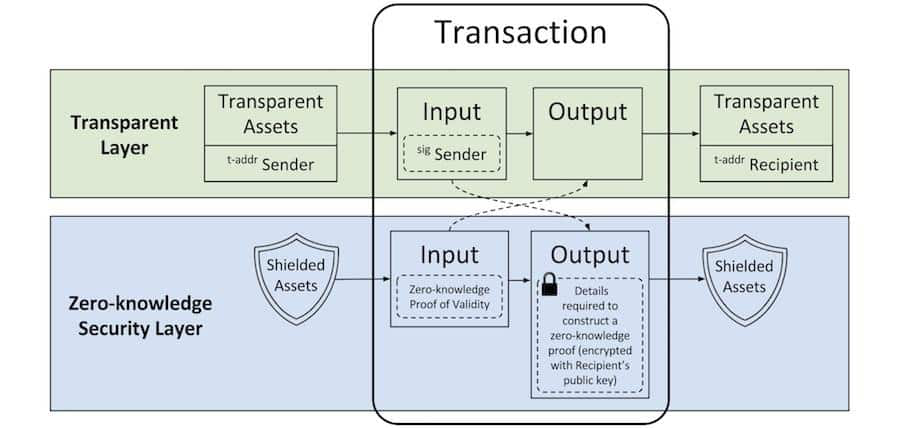
\includegraphics[width=1\linewidth]{img/zcashTransactions.png}
    \caption{Zcash Transaction}
    \label{fig:enter-label}
\end{figure}

\noindent In summary:
\begin{table}[!ht]
    \centering
    \begin{tabular}{>{\columncolor[gray]{0.9}}c|c|c}
        \toprule
        \rowcolor{gray!30}
        \textbf{Transaction Type} & \textbf{Privacy} & \textbf{Information Revealed} \\ \midrule
        Standard & Low & Sender, recipient, amount \\ \midrule
        Shielded & High & Sender, recipient, amount (hidden) \\ \bottomrule
    \end{tabular}
    \caption{Privacy levels of different transaction types}
    \label{tab:transaction_privacy}
\end{table}

\subsection{Sighash}

The \textbf{Sighash} is an essential component of the transaction signing mechanism in Zcash. It ensures that signed data has not been altered, protecting the transaction's integrity. It is a cryptographic hash calculated on specific elements of a transaction. This hash is then digitally signed to ensure the transaction cannot be modified without invalidating the signature.

\noindent The characteristics are as follows:
\begin{itemize}
    \item \textbf{Transaction structure}: as noted earlier, a Zcash transaction can contain multiple inputs, outputs, and, in the case of shielded transactions, zero-knowledge proofs;
    \item \textbf{Sighash calculation}: to create a signature, a hash (the sighash) of specific parts of the transaction is calculated. The digital signature is then created on this hash;
    \item \textbf{Types of Sighash}: Zcash inherits various types of sighash from Bitcoin, each with different implications for what is included in the hash calculation.
\end{itemize}

\noindent The sighash in shielded transactions must include the necessary elements to ensure critical data and zero-knowledge proofs have not been altered. The use of zk-SNARK proofs means that even the shielded parts of the transaction are included in the sighash calculation, ensuring private information is protected.

\noindent The different types of sighash are:
\begin{itemize}
    \item \textbf{SIGHASH-ALL}: signs the entire transaction. This is the most common type as it ensures no part of the transaction can be modified without invalidating the signature;
    \item \textbf{SIGHASH-NONE}: signs only the inputs, allowing modifications to the outputs without invalidating the signature. This type is less common as it offers less security;
    \item \textbf{SIGHASH-SINGLE}: signs only the corresponding input and output, allowing modifications to other inputs and outputs. Used in specific scenarios;
    \item \textbf{SIGHASH-ANYONECANPAY}: modifies the behavior of the previous sighashes by allowing anyone to add new inputs to the transaction without invalidating the original signature.
\end{itemize}

\noindent The hash algorithm used to calculate the sighash is the same as used by Bitcoin, i.e., SHA-256. More precisely, the hashing process involves a sequential double application of the algorithm, known as \textbf{double SHA-256}, to add an additional layer of security.

\noindent During the sighash calculation for a transaction, various fields of the transaction itself are included, such as inputs, outputs, and other metadata. The transaction is serialized, i.e., converted into a byte sequence, in a specific format. Only the fields necessary based on the sighash type (SIGHASH-ALL, SIGHASH-NONE, etc.) are included in the calculation. The hashing is then performed:
\begin{itemize}
    \item \textbf{First SHA-256}: the SHA-256 hash of the serialized data is calculated;
    \item \textbf{Second SHA-256}: the SHA-256 hash of the output of the first SHA-256 is calculated.
\end{itemize}

\noindent The resulting digest (sighash) is then digitally signed using the private key of the transaction's sender.